\documentclass[dvipdfmx,12pt]{beamer}
\usepackage{bxdpx-beamer}
\usepackage{pxjahyper}

\setbeamertemplate{navigation symbols}{}
\setbeamertemplate{footline}[frame number]

\usepackage{amssymb}
\usepackage{amsmath}
\usepackage{tikz}
\usepackage{mathtools}
\usepackage[absolute,overlay]{textpos}

\usetikzlibrary{positioning}
\usetikzlibrary{calc}
\usetikzlibrary{decorations.pathreplacing}

\newcommand{\scrN}{\mathcal{N}}
\newcommand{\scrC}{\mathcal{C}}
\newcommand{\scrI}{\mathcal{I}}
\newcommand{\scrJ}{\mathcal{J}}
\newcommand{\N}{\mathbb{N}}
\newcommand{\Z}{\mathbb{Z}}
\renewcommand{\P}{\mathbb{P}}
\newcommand{\Q}{\mathbb{Q}}
\newcommand{\R}{\mathbb{R}}
\newcommand{\C}{\mathbb{C}}
\newcommand{\range}{\operatorname{ran}}
\newcommand{\dom}{\operatorname{dom}}
\newcommand{\append}{{}^\frown}
\newcommand{\boldsig}{\boldsymbol{\Sigma}}
\newcommand{\boldpi}{\boldsymbol{\Pi}}
\newcommand{\bolddelta}{\boldsymbol{\Delta}}
\newcommand{\Ordinals}{\mathrm{On}}
\newcommand\forces{\Vdash}
\newcommand\notforces{\nVdash}
\newcommand{\cl}{\operatorname{cl}}
\newcommand{\intr}{\operatorname{int}}
\newcommand{\ro}{\operatorname{ro}}
\newcommand{\rank}{\operatorname{rank}}
\newcommand{\frakt}{\mathfrak{t}}
\newcommand{\s}{\mathfrak{s}}
\newcommand{\frakc}{\mathfrak{c}}
\newcommand{\frakd}{\mathfrak{d}}
\newcommand{\frakb}{\mathfrak{b}}
\newcommand{\frakv}{\mathfrak{v}}
\newcommand{\Pow}{\mathcal{P}}
\newcommand{\fin}{\mathrm{fin}}
\newcommand{\OR}{\mathbin{\text{または}}}
\newcommand{\AND}{\mathbin{\text{かつ}}}
\newcommand{\down}{\hspace{-0.2em}\downarrow}

\newcommand{\tukeyle}{\preceq_\mathrm{T}}
\newcommand{\non}{\operatorname{non}}
\newcommand{\cov}{\operatorname{cov}}
\newcommand{\add}{\operatorname{add}}
\newcommand{\cof}{\operatorname{cof}}
\newcommand{\nul}{\mathcal{N}}
\newcommand{\nll}{\mathcal{N}}
\newcommand{\meager}{\mathcal{M}}
\newcommand{\HDZ}{\mathrm{HDZ}}
\newcommand{\id}{\mathrm{id}}
\newcommand{\pow}{\operatorname{pow}}
\newcommand{\cf}{\operatorname{cf}}
\newcommand{\SAT}{\operatorname{SAT}}
\newcommand{\KT}{\operatorname{KT}}
\newcommand{\LangL}{\mathcal{L}}
\newcommand{\CH}{\mathrm{CH}}
\newcommand{\MA}{\mathrm{MA}}
\newcommand{\ZF}{\mathrm{ZF}}
\newcommand{\AD}{\mathrm{AD}}
\newcommand{\ZFC}{\mathrm{ZFC}}
\newcommand{\DC}{\mathrm{DC}}
\newcommand{\GP}{\operatorname{GP}}
\newcommand{\all}{\mathsf{all}}
\newcommand{\proj}{\operatorname{proj}}

\renewcommand\emptyset{\varnothing}
\renewcommand\subset{\subseteq}
\renewcommand{\setminus}{\smallsetminus}
\newcommand{\seq}[1]{{\langle#1\rangle}}

\DeclarePairedDelimiter\abs{\lvert}{\rvert}


\usepackage[backend=biber,style=alphabetic,sorting=nty,doi=false,isbn=false,url=false]{biblatex}
\addbibresource{bib.bib}
\nocite{*}
%\AtBeginBibliography{\scriptsize}

\renewcommand{\familydefault}{\sfdefault}  % 英文をサンセリフ体に
\renewcommand{\kanjifamilydefault}{\gtdefault}  % 日本語をゴシック体に
%\DeclareSymbolFont{operators}{OT1}{\sfdefault}{m}{n}
%\SetSymbolFont{operators}{bold}{OT1}{\sfdefault}{b}{n}
%\usefonttheme{structurebold} % タイトル部を太字
\setbeamerfont{alerted text}{series=\bfseries} % Alertを太字
%\setbeamerfont{section in toc}{series=\mdseries} % 目次は太字にしない
\setbeamerfont{frametitle}{size=\Large}
\setbeamerfont{title}{size=\huge}
\setbeamerfont{date}{size=\small}
\setbeamerfont{institute}{size=\small}
\setbeamerfont{author}{size=\large}

\definecolor{structcolordarker}{HTML}{6e396d}
%\definecolor{structcolor}{HTML}{B618F9}
\definecolor{structcolor}{HTML}{a856a7}
%\definecolor{structcolor}{HTML}{f0658e}
\definecolor{structcolorred}{HTML}{F70C0C}
\definecolor{blockcolor}{HTML}{B8B6C1}
\definecolor{theoremcolor}{HTML}{e5aec5}
\definecolor{lemmacolor}{HTML}{B3CEFF}
\definecolor{conjcolor}{HTML}{85BEDB}
\definecolor{deficolor}{HTML}{DBC7A8}
\definecolor{AlertOrange}{RGB}{235,56,0}
%\definecolor{AlmostBlack}{RGB}{38,38,38}
\definecolor{AlmostBlack}{RGB}{0,0,0}
%\definecolor{Pink}{HTML}{ffdedb}
\definecolor{Pink}{HTML}{FFC7C2}
\definecolor{Green}{HTML}{17b329}
\setbeamercolor{normal text}{fg=AlmostBlack}
\setbeamercolor{structure}{fg=structcolordarker}
\setbeamercolor{frametitle}{fg=structcolor!50!black, bg=structcolor!30!white}
%\setbeamercolor{frametitle}{fg=structcolor!0!white, bg=structcolor!70!black}
\setbeamercolor{block body}{bg=blockcolor!30!white}
\setbeamercolor{block title}{fg=blockcolor!10!black, bg=blockcolor!70!white}

%\setbeamercolor{title}{fg=white}

\newenvironment<>{thmblock}[1]{\begin{block}#2{#1}}{\end{block}}
\newenvironment<>{lemmablock}[1]{\begin{block}#2{#1}}{\end{block}}
\newenvironment<>{conjectureblock}[1]{\begin{block}#2{#1}}{\end{block}}
\newenvironment<>{defiblock}[1]{\begin{block}#2{#1}}{\end{block}}

\BeforeBeginEnvironment{thmblock}{
	\setbeamercolor{block body}{bg=theoremcolor!30!white}
	\setbeamercolor{block title}{fg=theoremcolor!0!black, bg=theoremcolor!100!white}
}
\AfterEndEnvironment{thmblock}{
	\setbeamercolor{block body}{bg=blockcolor!30!white}
	\setbeamercolor{block title}{fg=blockcolor!10!black, bg=blockcolor!70!white}
}
\BeforeBeginEnvironment{lemmablock}{
	\setbeamercolor{block body}{bg=lemmacolor!30!white}
	\setbeamercolor{block title}{fg=lemmacolor!0!black, bg=lemmacolor!100!white}
}
\AfterEndEnvironment{lemmablock}{
	\setbeamercolor{block body}{bg=blockcolor!30!white}
	\setbeamercolor{block title}{fg=blockcolor!10!black, bg=blockcolor!70!white}
}
\BeforeBeginEnvironment{conjectureblock}{
	\setbeamercolor{block body}{bg=conjcolor!30!white}
	\setbeamercolor{block title}{fg=conjcolor!0!black, bg=conjcolor!70!white}
}
\AfterEndEnvironment{conjectureblock}{
	\setbeamercolor{block body}{bg=blockcolor!30!white}
	\setbeamercolor{block title}{fg=blockcolor!10!black, bg=blockcolor!70!white}
}
\BeforeBeginEnvironment{defiblock}{
	\setbeamercolor{block body}{bg=deficolor!30!white}
	\setbeamercolor{block title}{fg=deficolor!0!black, bg=deficolor!100!white}
}
\AfterEndEnvironment{defiblock}{
	\setbeamercolor{block body}{bg=blockcolor!30!white}
	\setbeamercolor{block title}{fg=blockcolor!10!black, bg=blockcolor!70!white}
}

\setbeamercolor{alerted text}{fg=AlertOrange} % \alert 文字カラー

%フラットデザイン化
\setbeamertemplate{blocks}[rounded] % Blockの影を消す
\useinnertheme{circles} % 箇条書きをシンプルに
\setbeamertemplate{navigation symbols}{} % ナビゲーションシンボルを消す
\setbeamertemplate{footline}[frame number] % フッターはスライド番号のみ
\setbeamercolor{page number in head/foot}{fg=gray}

\setbeamertemplate{bibliography entry article}{}
\setbeamertemplate{bibliography entry title}{}
\setbeamertemplate{bibliography entry location}{}
\setbeamertemplate{bibliography entry note}{}
\setbeamertemplate{bibliography item}{\insertbiblabel}

\setbeamertemplate{itemize item}{\color{black}\textbullet}

\AtBeginSection[]{
	\begin{frame}
		\tableofcontents[currentsection]
	\end{frame}
}

\title{測度$0$集合の和集合に関するGoldsternの原理}
\author{後藤 達哉}
\institute{神戸大学}
\date{2022年9月15日 \\ 日本数学会2022年度秋季総合分科会 @ 北海道大学}

\begin{document}
	\maketitle
	
	\begin{frame}{測度$0$集合の和集合}
		$(Y, \mu)$をポーランド確率空間とする.
		測度の可算加法性より,測度$0$集合の可算個の和集合は再び測度$0$である.
		
		\vspace{0.5cm}
		Q. 連続体濃度個の測度$0$集合の和集合だとどうか?
		
		A. 必ずしも測度$0$ではない (たとえば:一点集合たちの和集合).
		
		\vspace{0.5cm}
		Q. 与えれた測度$0$集合たちに何か仮定を加えたらどうか?
		
		A. それをすると,連続体濃度個の測度$0$集合の和集合も測度$0$となる!
	\end{frame}
		
	\begin{frame}{Goldsternの定理}
		\begin{block}{}
			\textbf{(full domination order)} $x, x' \in \omega^\omega$について関係$x \le x'$を$(\forall n\in\omega)(x(n) \le x'(n))$で定める.
		\end{block}

			1993年,Martin Goldsternは次の定理を証明した.
				\begin{thmblock}{Goldsternの定理 ($\ZF+\DC$)}
					$(Y, \mu)$をポーランド確率空間とする.
					$A \subset \omega^\omega \times Y$を$\boldsig^1_1$集合とする.
					各$x \in \omega^\omega$について
					\[
					A_x := \{ y \in Y : (x, y) \in A \}
					\]
					が測度$0$だと仮定する.
					また$(\forall x, x' \in \omega^\omega)(x \le x' \Rightarrow A_{x} \subset A_{x'})$を仮定する.
					このとき$\bigcup_{x \in \omega^\omega} A_x$も測度$0$である.
				\end{thmblock}
	\end{frame}

	\begin{frame}{原理$\GP(\Gamma)$}
		\begin{defiblock}{定義}
			$\Gamma$をポイントクラスとする.
			このとき\alert{$\GP(\Gamma)$}とは次の主張である:
			$(Y, \mu)$をポーランド確率空間とし$A \subset \omega^\omega \times Y$は$\Gamma$に属するとする.
			各$x \in \omega^\omega$について$A_x$は測度$0$だとする.
			また$(\forall x, x' \in \omega^\omega)(x \le x' \Rightarrow A_{x} \subset A_{x'})$だとする.
			すると$\bigcup_{x \in \omega^\omega} A_x$も測度$0$である.
		\end{defiblock}
	
		Goldsternの定理は$\GP(\boldsig^1_1)$が成り立つことを主張している.
	\end{frame}

	\begin{frame}{主結果}
		記号``$\all$"はポーランド空間のすべての部分集合のなすクラスを表す.
		\begin{thmblock}{定理}
			$\GP(\all)$は$\ZFC$から独立している.
		\end{thmblock}
		
	\end{frame}
		
	\begin{frame}{$\neg \GP(\all)$の無矛盾性}
		\begin{columns}
			\begin{column}{0.58\textwidth}
				\begin{thmblock}{定理}
					$\CH$を仮定すると$\neg \GP(\all)$が導かれる.
				\end{thmblock}
				証明.$\seq{x_\alpha : \alpha < \omega_1}$を$(\omega^\omega, <^*)$の共終単調増加列とする.$\seq{y_\alpha : \alpha < \omega_1}$を$2^\omega$の元の枚挙とする.
				すると次で定まる集合$A$は$\neg \GP(\all)$の証拠である:
				\[
				A_x = \{ y_\beta : \beta < \alpha_x  \},
				\]
				ここで$\alpha_x = \min \{\alpha : x <^* x_\alpha \}$. \qed
			\end{column}
			\begin{column}{0.48\textwidth}
				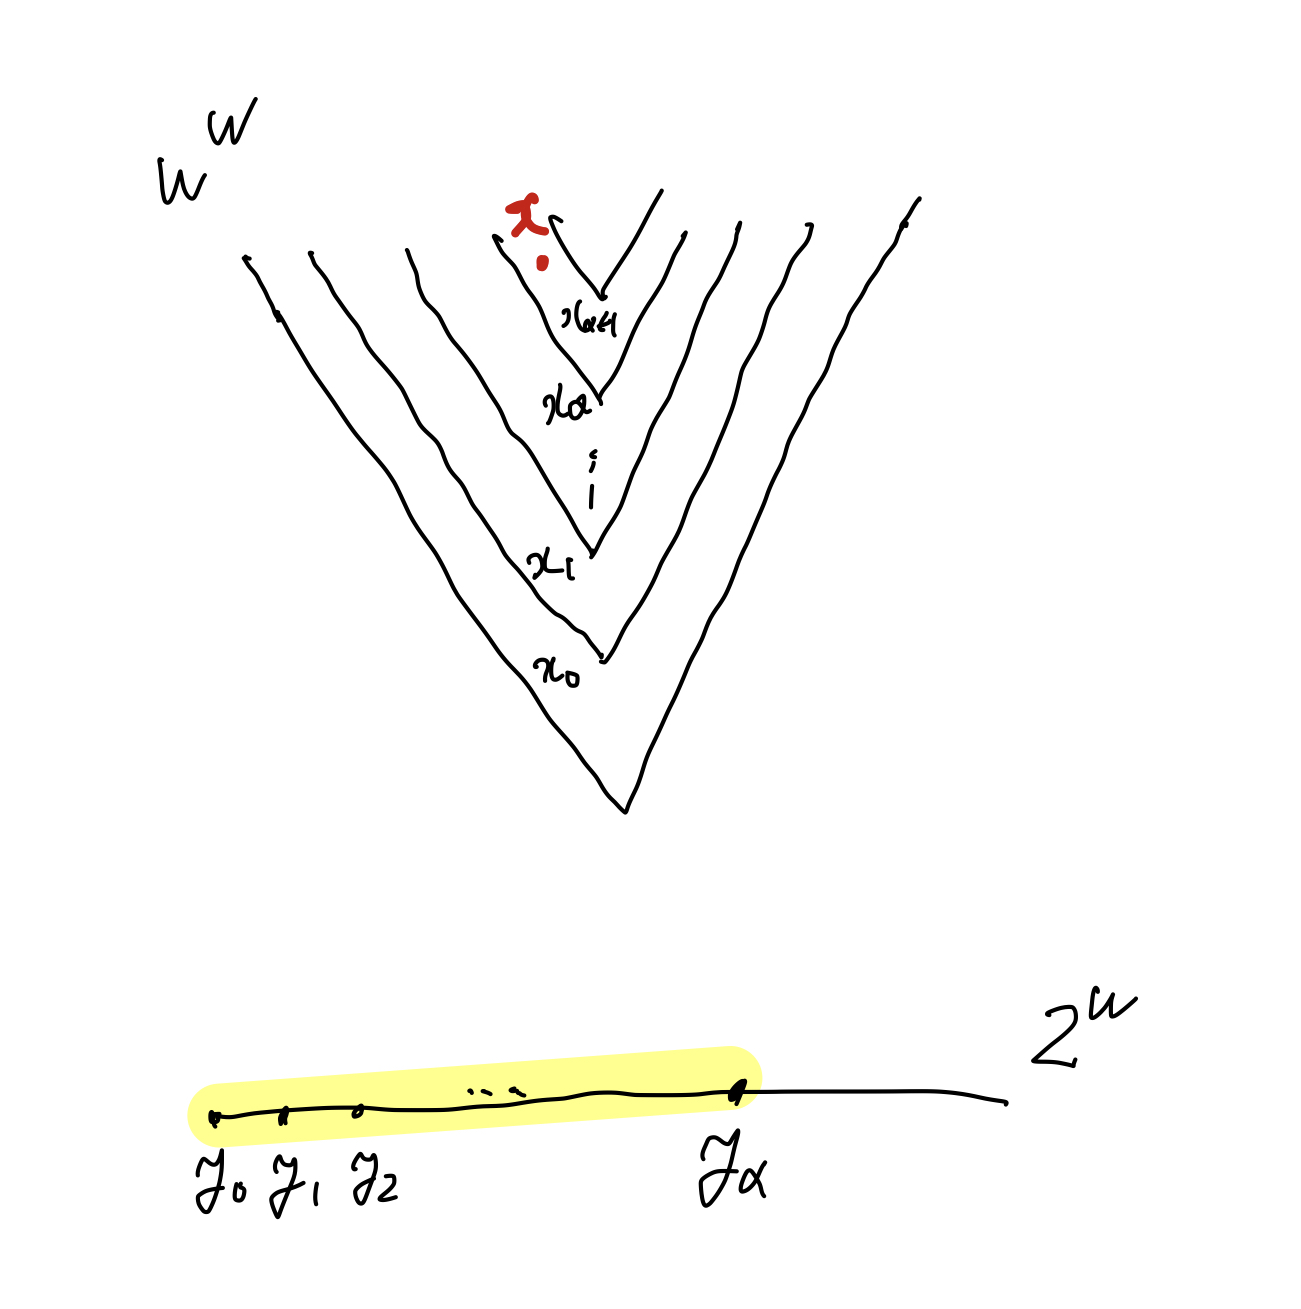
\includegraphics[width=5.5cm]{IMG_0149.jpg}
			\end{column}
		\end{columns}
	\end{frame}

	\begin{frame}{$\neg \GP(\all)$の無矛盾性}
		最後の証明を改良すると次の定理も得られる.
	\begin{thmblock}{定理}
		次の3つの条件のうち少なくとも1つが成立すると仮定する.

		\hspace{2em}$\add(\nul) = \frakb$, $\non(\nul) = \frakb$ or $\non(\nul) = \frakd$.
		
		すると$\neg \GP(\all)$が成り立つ.
	\end{thmblock}
	\begin{block}{}
	{\scriptsize
		$\add(\nul) := \min \{ \kappa : \text{the null ideal is not } \kappa\text{-additive} \}$
		$\non(\nul) := \min \{ \abs{A} : A \subset 2^\omega, A \text{ does not have measure } 0 \}$
		$\frakb := \min \{ \abs{F} : F \subset \omega^\omega, \neg (\exists g \in \omega^\omega)(\forall f \in F) \ f <^* g \}$
		$\frakd := \min \{ \abs{F} : F \subset \omega^\omega, (\forall g \in \omega^\omega)(\exists f \in F) \ g <^* f \}$
	}
	\end{block}
	\end{frame}

	\begin{frame}{$\neg \GP(\all)$の無矛盾性}
	\begin{thmblock}{}
		次の3つの条件のうち少なくとも1つが成立すると仮定する:
		$\add(\nul) = \frakb$, $\non(\nul) = \frakb$ or $\non(\nul) = \frakd$.
		すると$\neg \GP(\all)$が成り立つ.
	\end{thmblock}
	\begin{block}{}
		{\scriptsize
			$\add(\nul) := \min \{ \kappa : \text{the null ideal is not } \kappa\text{-additive} \}$
			$\non(\nul) := \min \{ \abs{A} : A \subset 2^\omega, A \text{ does not have measure } 0 \}$
			$\frakb := \min \{ \abs{F} : F \subset \omega^\omega, \neg (\exists g \in \omega^\omega)(\forall f \in F) \ f <^* g \}$
			$\frakd := \min \{ \abs{F} : F \subset \omega^\omega, (\forall g \in \omega^\omega)(\exists f \in F) \ g <^* f \}$
		}
	\end{block}

	\[
	\begin{tikzpicture}
		\tikzset{
			textnode/.style={text=black},
		}
		\tikzset{
			edge/.style={color=black,thick},
		}
		\newcommand{\w}{2}
		\newcommand{\h}{1}
		
		\node[textnode] (addN) at (0, 0) {$\add(\nll)$};
		\node[textnode] (covN) at (0, \h*2) {$\cov(\nll)$};
		
		\node[textnode] (addM) at (\w, 0) {$\add(\meager)$};
		\node[textnode] (b) at (\w, \h) {$\mathfrak{b}$};
		\node[textnode] (nonM) at (\w, \h*2) {$\non(\meager)$};
		
		\node[textnode] (covM) at (\w*2, 0) {$\cov(\meager)$};
		\node[textnode] (d) at (\w*2, \h) {$\mathfrak{d}$};
		\node[textnode] (cofM) at (\w*2, \h*2) {$\cof(\meager)$};
		
		\node[textnode] (nonN) at (\w*3, 0) {$\non(\nll)$};
		\node[textnode] (cofN) at (\w*3, \h*2) {$\cof(\nll)$};
		
		\node[textnode] (aleph1) at (-\w, 0) {$\aleph_1$};
		\node[textnode] (c) at (\w*4, \h*2) {$2^{\aleph_0}$};
		
		\draw[->,edge] (addN) to (covN);
		\draw[->,edge] (addN) to (addM);
		\draw[->,edge] (covN) to (nonM);	
		\draw[->,edge] (addM) to (b);
		\draw[->,edge] (b) to (nonM);
		\draw[->,edge] (addM) to (covM);
		\draw[->,edge] (nonM) to (cofM);
		\draw[->,edge] (covM) to (d);
		\draw[->,edge] (d) to (cofM);
		\draw[->,edge] (b) to (d);
		\draw[->,edge] (covM) to (nonN);
		\draw[->,edge] (cofM) to (cofN);
		\draw[->,edge] (nonN) to (cofN);
		\draw[->,edge] (aleph1) to (addN);
		\draw[->,edge] (cofN) to (c);
	\end{tikzpicture}
	\]

	\end{frame}

	\begin{frame}{$V=L$は$\neg \GP(\Delta^1_2)$を含意する}
		最後の定理の証明を別の方法で改良すると,次の定理も得られる.
		\begin{thmblock}{定理}
			$V=L$は$\neg \GP(\Delta^1_2)$を導く.
		\end{thmblock}
	\end{frame}

	\begin{frame}{$\GP(\all)$の無矛盾性}
	\begin{thmblock}{定理}
		$\ZFC$が無矛盾ならば$\ZFC + \GP(\all)$も無矛盾である.
	\end{thmblock}
	実際,``Laverモデル"が$\GP(\all)$のモデルである.
	
	
	\[
	\begin{tikzpicture}
		\tikzset{
			textnode/.style={text=black},
		}
		\tikzset{
			edge/.style={color=black,thick},
		}
		\newcommand{\w}{2}
		\newcommand{\h}{1}
		
		\fill[color=white!80!cyan] (-\w*1.2,\h*2.5) rectangle (\w*4.3, -\h*0.5);
		\fill[color=white!60!blue] (\w/2,\h*2.5) rectangle (\w*4.3, \h*0.5);
		
		\node[textnode] at (0, -\h) {\color{cyan}equal to $\aleph_1$ in the Laver model};
		\node[textnode] at (\w*2.5, \h*3) {\color{blue}equal to $\aleph_2$ in the Laver model};
		
		\node[textnode] (addN) at (0, 0) {$\add(\nll)$};
		\node[textnode] (covN) at (0, \h*2) {$\cov(\nll)$};
		
		\node[textnode] (addM) at (\w, 0) {$\add(\meager)$};
		\node[textnode] (b) at (\w, \h) {$\mathfrak{b}$};
		\node[textnode] (nonM) at (\w, \h*2) {$\non(\meager)$};
		
		\node[textnode] (covM) at (\w*2, 0) {$\cov(\meager)$};
		\node[textnode] (d) at (\w*2, \h) {$\mathfrak{d}$};
		\node[textnode] (cofM) at (\w*2, \h*2) {$\cof(\meager)$};
		
		\node[textnode] (nonN) at (\w*3, 0) {$\non(\nll)$};
		\node[textnode] (cofN) at (\w*3, \h*2) {$\cof(\nll)$};
		
		\node[textnode] (aleph1) at (-\w, 0) {$\aleph_1$};
		\node[textnode] (c) at (\w*4, \h*2) {$2^{\aleph_0}$};
		
		\draw[->,edge] (addN) to (covN);
		\draw[->,edge] (addN) to (addM);
		\draw[->,edge] (covN) to (nonM);	
		\draw[->,edge] (addM) to (b);
		\draw[->,edge] (b) to (nonM);
		\draw[->,edge] (addM) to (covM);
		\draw[->,edge] (nonM) to (cofM);
		\draw[->,edge] (covM) to (d);
		\draw[->,edge] (d) to (cofM);
		\draw[->,edge] (b) to (d);
		\draw[->,edge] (covM) to (nonN);
		\draw[->,edge] (cofM) to (cofN);
		\draw[->,edge] (nonN) to (cofN);
		\draw[->,edge] (aleph1) to (addN);
		\draw[->,edge] (cofN) to (c);
	\end{tikzpicture}
	\]
	\end{frame}

	\begin{frame}{$\boldsig^1_2$正則性との関係}
		\begin{thmblock}{定理}
			$\boldsig^1_2$ Lebesuge可測性は$\GP(\boldsig^1_2)$を導く.
			さらに$\GP(\bolddelta^1_2)$は任意の実数$a$に対して$L[a]$上のdominating実数があることを導く.
		\end{thmblock}
		\[
	\begin{tikzpicture}[scale=0.7]
	\node (sigma12lm) at (0, 0) {$\boldsig^1_2$-LM};
	\node (sigma12bp) at (3, 0) {$\boldsig^1_2$-BP};
	\node[align=left] (dominating) at (10, 0) {$(\forall a \in \R)(\exists z \in \omega^\omega)$ \\ \hspace{0.5cm}$(\text{$z$ is a dominating real over $L[a]$})$};
	\node (gpsigma12) at (1.5, -2) {$\GP(\boldsig^1_2)$};
	\node (gpdelta12) at (4.5, -2) {$\GP(\bolddelta^1_2)$};
	
	\draw[->] (sigma12lm) -> (sigma12bp);
	\draw[->] (sigma12bp) -> (dominating);
	\draw[->] (sigma12lm) -> (gpsigma12);
	\draw[->] (gpsigma12) -> (gpdelta12);
	\draw[->] (gpdelta12) -> (dominating);
\end{tikzpicture}
\]
	\end{frame}

	\begin{frame}{決定性とSolovayモデル}
		\begin{thmblock}{定理}
			$\ZF + \AD$を仮定すると$\GP(\all)$が成り立つ.
		\end{thmblock}
		\begin{thmblock}{定理}
			Solovayモデルにおいて$\GP(\all)$が成り立つ.
		\end{thmblock}
	\end{frame}

	\begin{frame}{まとめ}
		\begin{itemize}
			\item Goldsternは$\GP(\boldsig^1_1)$を証明した.
			\item 我々は次を証明した:
			\begin{enumerate}
				\item $\GP(\all)$が$\ZFC$から独立している.
				\item $V=L$が$\neg \GP(\Delta^1_2)$を導く.
				\item $\ZF+\AD$が$\GP(\all)$を導く.
				\item Solovayモデルで$\GP(\all)$が成り立つ.
			\end{enumerate}
		\end{itemize}
	\end{frame}
	
	\begin{frame}{未解決問題}
	\begin{enumerate}
		\item $V=L$は$\neg \GP(\Pi^1_1)$を導くか?	
		\item $\ZFC+(\frakc>\aleph_2)+\GP(\all)$は無矛盾か?
		\item (到達不能基数を仮定して)$\ZF$のモデルで実数の任意の集合がLebesgue可測だが,$\GP(\all)$を満たさないものはあるか?
		\item ある$n \ge 2$	(または全ての$n \ge 2$)について,$\GP(\Sigma^1_{n+1})$と$\GP(\Sigma^1_n)$を分離することは,巨大基数を使わずにできるか?
	\end{enumerate}
	\end{frame}

	\begin{frame}{参考文献と謝辞}
		\printbibliography

		\vspace{0.5cm}

		この研究のプレプリント:arXiv:2206.08147

		\vspace{0.5cm}

		この研究において吉信康夫氏,木原貴行氏,Jörg Brendle氏,池上大祐氏,Martin Goldstern氏に助言を頂いた.

		\vspace{0.5cm}
		本研究はJSPS科研費 JP22J20021の助成を受けたものである.
	\end{frame}	
\end{document}